\documentclass[11pt,a4paper]{article}
\usepackage[margin=1in]{geometry}
\usepackage{graphicx}
\usepackage{amsmath,amssymb}
\usepackage{cite}
\usepackage{hyperref}
\usepackage{setspace}
\usepackage{titlesec}
\usepackage{caption}

\titleformat{\section}{\normalfont\large\bfseries}{\thesection}{1em}{}
\titleformat{\subsection}{\normalfont\normalsize\bfseries}{\thesubsection}{1em}{}

\onehalfspacing

\title{\textbf{An Integrated Machine Learning Framework for Biomolecule Design and Bioprocess Monitoring: A Mini Project Proposal}}
\author{Abu Henaf Rashid Ahmad Mufti \\ Biotechnology Internship \\ CodeAlpha}
\date{\today}

\begin{document}

\maketitle

\begin{abstract}
\noindent This proposal outlines a mini research project that examines how generative and predictive machine learning models are reshaping two connected stages of biotechnology work: the computational design of biomolecules and the real-time monitoring of biomanufacturing processes. Drawing on recent work in generative RNA aptamer evolution, protein-language-model-guided CRISPR engineering, and convolutional neural network based spectroscopic quality control, the project proposes a small-scale demonstration pipeline that mirrors these three stages using public or synthetic datasets. The intent is not to reproduce any single paper's full experimental scale, but to build a working, testable version of the underlying computational logic and evaluate it against reported benchmarks where feasible.
\end{abstract}

\section{Introduction}

Biotechnology research has quietly stopped being just a wet-lab discipline. Over the past two or three years, generative sequence models, protein language models, and spectroscopy-coupled neural networks have moved from proof-of-concept papers into workflows that actually replace multi-round experimental screening. The shift is visible across three fairly different problems: designing RNA aptamers that bind a target protein, engineering CRISPR-Cas enzymes to recognize new genomic sites, and monitoring antibody quality during large-scale purification. All three used to depend on slow, iterative laboratory cycles. All three now have a machine learning model sitting somewhere in the loop, either replacing rounds of screening outright or predicting a property in seconds that used to take a chromatography run to measure.

What ties these together, at least from a computational point of view, is not the biology itself but the pattern: a model learns a representation of sequence or spectral data, gets guided by some activity or quality signal, and either generates new candidates or predicts a property directly. That pattern is general enough that a student project can build a scaled-down version of it without needing a wet lab, which is the premise this proposal works from.

\section{Problem statement}

Three recurring bottlenecks show up across current biotechnology pipelines:

\begin{enumerate}
\item \textbf{Slow iterative discovery.} Traditional aptamer selection (SELEX) and directed protein evolution both rely on repeated rounds of screening, amplification, and re-screening. Each round can take weeks, and there is no guarantee that additional rounds converge on a genuinely optimal candidate rather than whatever survived selection pressure that particular week.
\item \textbf{Structural blindness in protein engineering.} Many CRISPR-Cas variants of interest lack solved crystal structures, so engineering approaches that depend on structural data cannot be applied to them. A sequence-only approach is needed for these enzymes to be engineered at all.
\item \textbf{Lag between manufacturing and quality assessment.} In biopharmaceutical production, critical quality attributes such as antibody charge variant distribution are typically measured offline using chromatography, which means a batch can move well past the point where a correction could have been made before the result comes back.
\end{enumerate}

None of these are new problems. What is new is that ML models are now accurate enough, on real experimental data, to be used as a practical substitute for parts of the traditional pipeline rather than just an academic curiosity.

\section{Objectives}

The project has four objectives:

\begin{enumerate}
\item Implement a simplified generative sequence model, structured as a conditional autoencoder over nucleotide or amino acid sequences, capable of proposing new candidate sequences conditioned on a target activity score.
\item Implement a lightweight in-silico mutagenesis routine that scores single-residue or single-nucleotide substitutions against a trained predictive model, to identify positions that matter most for a target property.
\item Implement a one-dimensional convolutional neural network that maps spectral-style input (real spectra if accessible, otherwise simulated spectra with controlled noise) to a continuous quality attribute, and benchmark it against a simple regression baseline.
\item Evaluate all three components on held-out data using standard metrics (accuracy, Pearson correlation, RMSE where relevant) and document where the scaled-down version diverges from the reported literature results, being explicit about what was necessarily simplified.
\end{enumerate}

\section{Methodology}

The project is organized into three modules that mirror the three bottlenecks above. Each module is described with its data source, model architecture, and evaluation plan.

\subsection{Module 1: Generative sequence design}

This module is modeled loosely on the GRAPE-LM approach to one-round RNA aptamer evolution \cite{grapelm}, which combines a transformer-based conditional autoencoder with an activity-guidance signal derived from screening data, rather than relying on repeated SELEX rounds.

\begin{figure}[h]
\centering
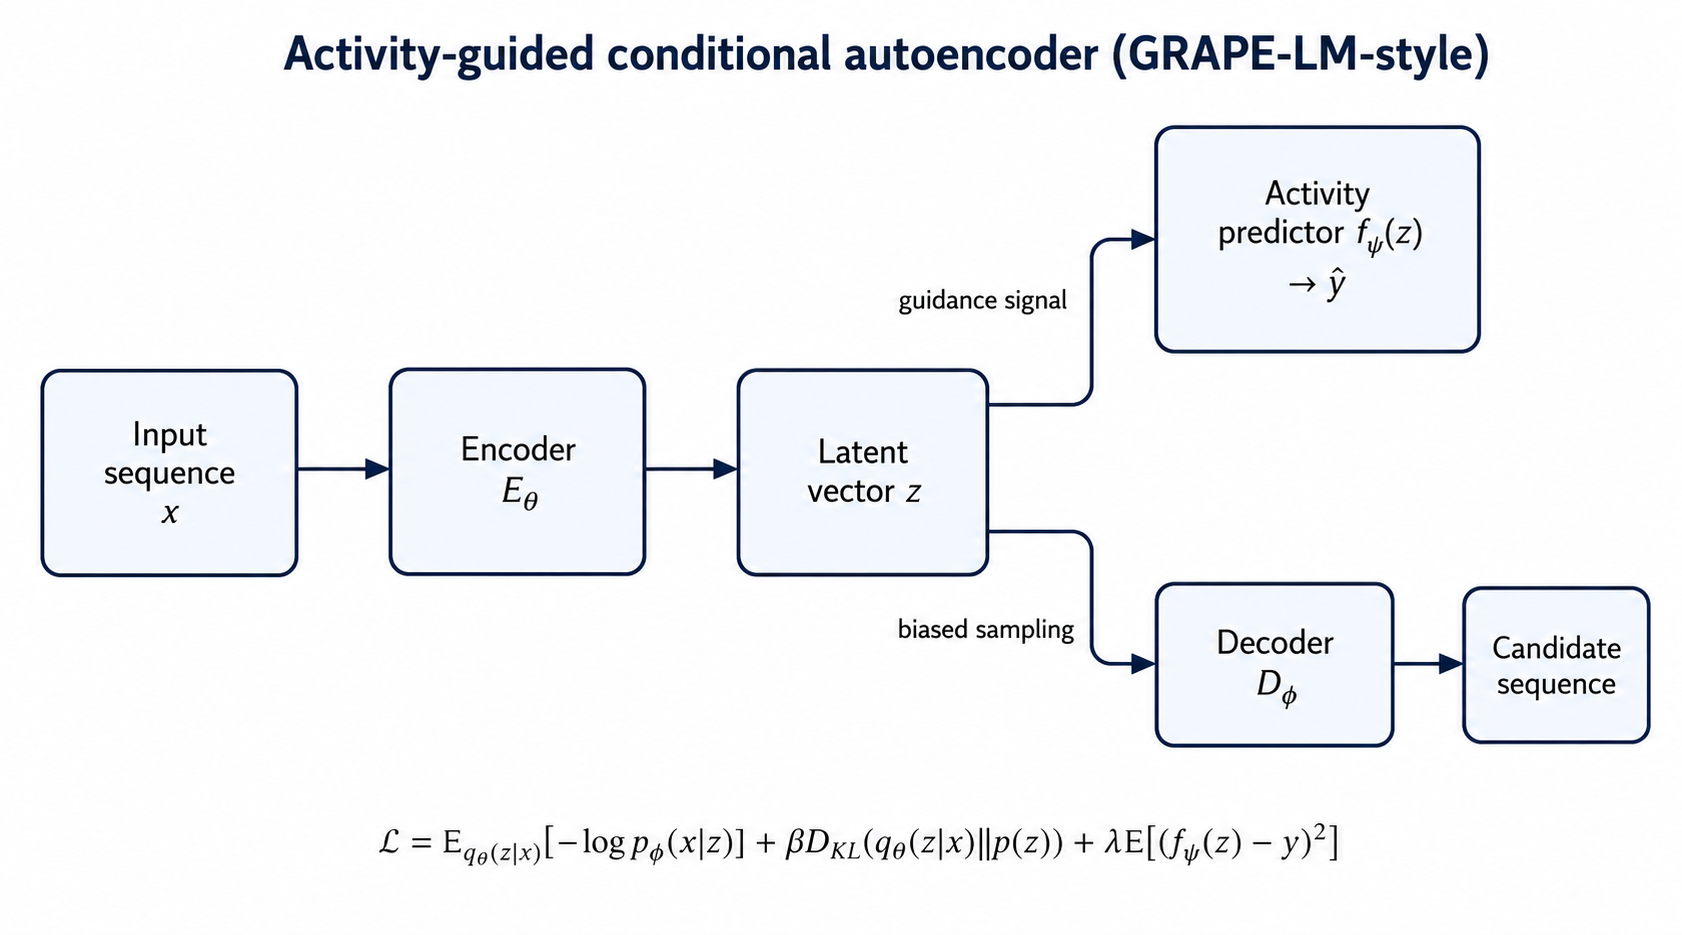
\includegraphics[width=0.75\textwidth]{Generative_pipeline_diagram.png}
\caption{Overview of the conditional autoencoder pipeline, from sequence encoding to activity-guided latent sampling and decoding.}
\end{figure}

The sequence encoder $E_\theta$ maps an input sequence $x$ to a latent vector $z$, and a decoder $D_\phi$ reconstructs the sequence from $z$. An auxiliary activity predictor $f_\psi(z)$ is trained jointly to regress a measured activity score $y$ from the same latent space, so that the latent space organizes itself by function and not just by sequence similarity. The combined training objective is:

\begin{equation}
\mathcal{L}(\theta,\phi,\psi) = \underbrace{\mathbb{E}_{q_\theta(z|x)}[-\log p_\phi(x|z)]}_{\text{reconstruction}} + \beta \, D_{KL}\big(q_\theta(z|x) \,\|\, p(z)\big) + \lambda \, \mathbb{E}\big[(f_\psi(z) - y)^2\big]
\end{equation}

where $\beta$ weights the KL regularization term against a standard normal prior $p(z)$, and $\lambda$ weights the activity-guidance loss. Once trained, new candidate sequences are generated by sampling latent vectors biased toward the high-activity region of the latent space and decoding them back into sequence.

For a course-scale version of this, the plan is to use a public aptamer or short-sequence dataset (for example, SELEX round data available from prior published studies) rather than generating new wet-lab data, and to treat the activity label as whatever binding or enrichment score the dataset provides.

\subsection{Module 2: In-silico mutagenesis for property-critical residues}

This module follows the logic of Protein2PAM \cite{protein2pam}, an evolution-informed protein language model trained on over 45{,}000 CRISPR-Cas PAM sequences to predict PAM specificity directly from protein sequence, without relying on structural data. The original work used deep mutational scanning to identify PAM-specifying mutations, defined as single residue changes that shift the predicted PAM distribution by a meaningful margin.

For a smaller version of this, a pretrained protein language model embedding is used as input to a lightweight classifier or regressor $g_\omega$ that predicts a target property (in the original work, PAM identity; in a scaled-down replication, this could be a simpler labeled property from a public protein dataset). Mutational sensitivity for position $i$ is then estimated as:

\begin{equation}
\Delta_i = \Big| g_\omega\big(\text{seq}\big) - \mathbb{E}_{a \in \mathcal{A}}\big[g_\omega(\text{seq}_{i \to a})\big] \Big|
\end{equation}

where $\text{seq}_{i \to a}$ denotes the sequence with position $i$ substituted by amino acid $a$, and $\mathcal{A}$ is the set of twenty standard amino acids. Positions with high $\Delta_i$ are flagged as candidate residues for guided variant design, following the same logic used to computationally evolve Nme1Cas9 variants with broadened PAM recognition in the source paper.

\subsection{Module 3: Spectral quality prediction with a 1D-CNN}

This module is based on the use of Raman spectroscopy combined with convolutional neural networks for real-time prediction of monoclonal antibody charge variant distribution during cation exchange chromatography \cite{ramancnn}. In the original study, Raman spectra collected across a reference library of samples with known acidic, main, and basic species distributions were used to train a CNN that predicts charge variant composition directly from spectral input, replacing an offline chromatography measurement.

\begin{figure}[h]
\centering
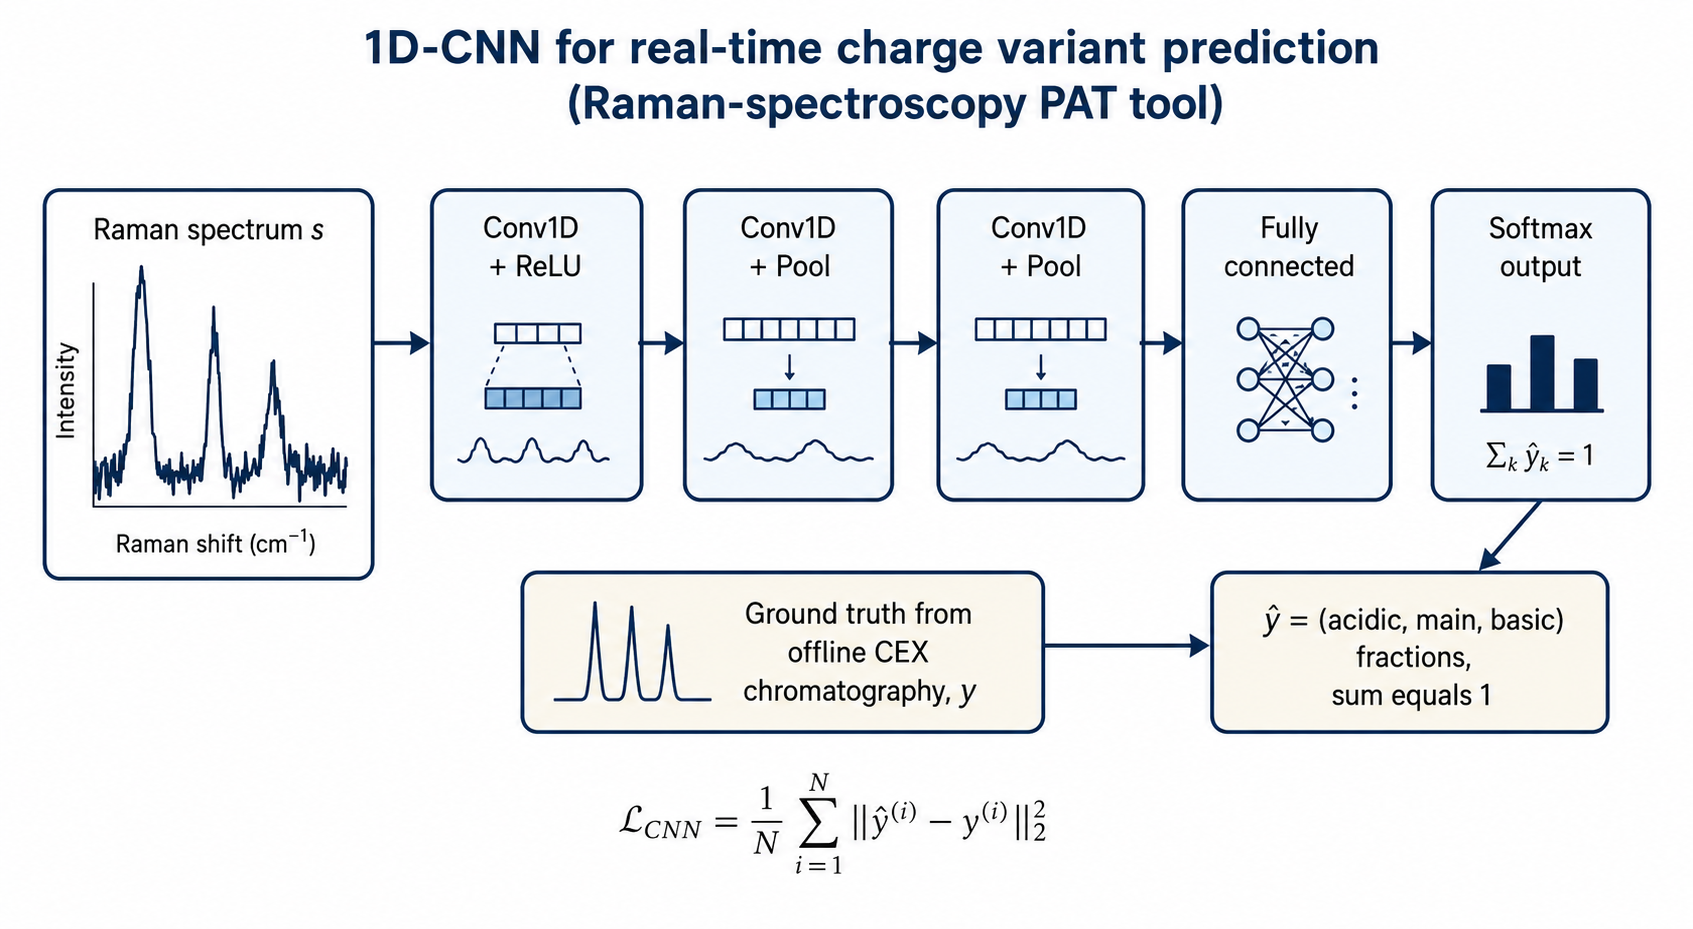
\includegraphics[width=0.75\textwidth]{CNN_spectral_architecture.png}
\caption{1D-CNN architecture mapping Raman spectral input to predicted charge variant proportions.}
\end{figure}

For a 1D spectral input $s \in \mathbb{R}^n$, the CNN applies a sequence of convolutional and pooling layers followed by fully connected layers to output a predicted composition vector $\hat{y} \in \mathbb{R}^3$ (acidic, main, basic fractions), constrained to sum to one via a softmax output layer:

\begin{equation}
\hat{y}_k = \frac{\exp(z_k)}{\sum_{j=1}^{3} \exp(z_j)}, \qquad k \in \{\text{acidic, main, basic}\}
\end{equation}

Training minimizes mean squared error between predicted and chromatography-measured composition:

\begin{equation}
\mathcal{L}_{\text{CNN}} = \frac{1}{N} \sum_{i=1}^{N} \| \hat{y}^{(i)} - y^{(i)} \|_2^2
\end{equation}

Since access to proprietary Raman spectral libraries is unlikely, the plan is to either use a public Raman dataset for a related regression task or generate synthetic mixture spectra with controlled noise, an approach comparable to the RaMix-style synthetic benchmarking used in related bioprocess ML work, to at least validate that the architecture and training loop behave correctly on data with known ground truth.

\subsection{Evaluation plan}

Each module is evaluated separately, since they operate on different data types and are not expected to be combined into a single end-to-end system at this scale:

\begin{itemize}
\item Module 1: reconstruction accuracy on held-out sequences, and correlation between predicted and true activity scores for the auxiliary predictor.
\item Module 2: classification or regression accuracy of $g_\omega$ on held-out labeled proteins, and a qualitative check of whether flagged high-$\Delta_i$ positions correspond to biologically plausible functional regions where such annotation is available.
\item Module 3: RMSE and Pearson correlation between predicted and true composition fractions on a held-out test split, compared against a simple partial least squares regression baseline, since prior bioprocess ML literature has shown PLS remains competitive on smaller datasets.
\end{itemize}

\section{Expected outcome}

The project is expected to produce three working, documented model implementations rather than a single unified system, since the underlying data types (sequence, protein embedding, spectral) do not naturally combine at this scale. For Module 1, a reasonable outcome is a generative model that can propose sequences enriched for a target property compared to random sequences, even if it does not match the reported performance of the full GRAPE-LM system trained on CRISPR-Cas-based intracellular screening data. For Module 2, the expected outcome is a working mutational sensitivity map that at least qualitatively agrees with known functional regions in the test protein, without claiming the precision of the original 45,000-sequence trained model. For Module 3, the CNN is expected to outperform a naive baseline on synthetic or public spectral data, demonstrating that the architecture is sound even without access to the original proprietary chromatography dataset.

Beyond the models themselves, the project should produce a clear, honest comparison between what a course-scale replication can achieve and what the original published systems report, along with a discussion of where the gap comes from: mostly dataset size and access to wet-lab-generated activity labels, rather than any fundamental flaw in the modeling approach.

% Acknowledgment with enumeration i), ii), iii)
\section*{Acknowledgment}

\noindent The author used AI tools for language editing and
formatting assistance. Figures were also generated with the aid of AI for precise display. All content and data
are the authors' own work.

\vspace{4pt} % a little space after the items

% 


\begin{thebibliography}{9}

\bibitem{panjwani}
J. Panjwani, ``Artificial intelligence and machine learning-assisted digital applications for biopharmaceutical manufacturing,'' \emph{Biotechnology Progress}, vol. 42, no. 2, p. e70089, 2026.

\bibitem{grapelm}
J. Zhang, J. Zhang, and Y. Wang, ``Combining generative AI and one round of wet lab evolution generates high-affinity RNA aptamers,'' \emph{Nature Biotechnology}, Feb. 2026.

\bibitem{protein2pam}
S. Nayfach, A. Bhatnagar, A. Novichkov, \emph{et al.}, ``Customizing CRISPR--Cas PAM specificity with protein language models,'' \emph{Nature Biotechnology}, Feb. 2026.

\bibitem{ramancnn}
Authors not fully listed in available source, ``Convolutional neural networks guided Raman spectroscopy as a process analytical technology (PAT) tool for monitoring and simultaneous prediction of monoclonal antibody charge variants,'' \emph{Pharmaceutical Research}, Feb. 2024.

\bibitem{review2025}
Authors not fully listed in available source, ``Machine learning in biological research: key algorithms, applications, and future directions,'' \emph{PMC}, 2025.

\bibitem{phillip2025}
A. Phillip, ``The role of artificial intelligence in modern biotechnology: a comprehensive review,'' \emph{Journal of Applied Biotechnology Reports}, vol. 13, no. 1, pp. 1899--1921, 2025.

\bibitem{bibliometric}
D. Xu \emph{et al.}, ``Bibliometric analysis of artificial intelligence for biotechnology and applied microbiology: exploring research hotspots and frontiers,'' \emph{Frontiers in Bioengineering and Biotechnology}, vol. 10, p. 998298, 2022.

\end{thebibliography}

\end{document}
